\subsection{Calibrating a new gyrochronology relation}
\label{sec:calibration}

We used a two-dimensional power-law relation, augmented with a Gaussian
process, as our new empirical gyrochronology model.
This model was fitted to kinematic ages (described above) and open cluster
stars with precise rotation periods measured from Kepler and K2 light curve
and well-determined ages from cluster-based isochrone fitting.
In this section we describe the model, and how we fit it to the data, in more
detail.

\subsubsection{The Model}

To calibrate a new empirical gyrochronology relation
we used a composite model, consisting of an underlying mean function,
augmented with a Gaussian process.
The mean function is similar to previous empirical gyrochronology models and
consists of two separable power-law relations: one describing the relationship
between rotation period and age, and the other the relationship between
rotation period and color \citep[\eg][]{barnes2003, barnes2007, mamajek2008,
meibom2015, angus2015, angus2019}.

Our mean function is comprised of a single power-law in age, $f(t)$, and a
broken power law in color, $g(C)$:
\begin{equation}
P_\mathrm{rot} = f(t) g(C),
\end{equation}
where $P_\mathrm{rot}$ is rotation period in days, $t$ is age in Gyr, and $C$
is Gaia color, \gcolor.
The age power-law is defined as,
\begin{equation}
f(t) = at^n,
\end{equation}
following the functional form first described in \citet{barnes2003}, where $a$
and $n$ are free parameters.
The broken power-law in color is defined as,
\begin{equation}
    g(C) = \left[
\left(\frac{m_1}{1 + e^{s \delta}}\right)
    + \left(\frac{m_2}{1 + e^{-s \delta}}\right)\right]^\delta,
\end{equation}
where $s$ is a parameter that determines how smooth the break is, $m_1$ is the
slope below (bluewards of) the power-law break, $m_2$ is the slope above
(redwards of) the break, and
\begin{equation}
\delta = C - C_\mathrm{break},
\end{equation}
where $C_\mathrm{break}$ is the color of the power-law break.
In this model, $s$, $m_1$, $m_2$, and $C_\mathrm{break}$ are all free
parameters.

We used a Gaussian process model to `distort' this mean model, providing a
better fit to the data.
The GP models the residuals between the mean model and the data.
We used a simple squared exponential kernel function which has only two free
parameters, an amplitude, $A$ and a length scale, $l$.
This kernel function is defined as,
\begin{equation}
k_{ij} = A \exp\left[{\frac{-(x_i - x_j)^2}{2l^2}}\right]
\end{equation}

The parameters were optimized using the {\tt exoplanet} code \citep{exoplanet}.
% The posterior PDFs of these parameters of the power-law relations, and the
% hyper-parameters of the GP kernel were explored with MCMC.
% We used the {\tt exoplanet} \citep{exoplanet} and {\tt PyMC3} \citep{pymc3}
% Python packages to fit this model to the data.

\subsubsection{Formatting the data}

A Gaussian process is only an appropriate model for data generated by a
Gaussian process.
Data with large numbers of outliers or with inaccurately estimated
uncertainties are not Gaussian-distributed and therefore cannot be described
with a Gaussian process.
Rotation period measurements are rarely generated by a Gaussian process for
two main reasons.
Firstly, the uncertainties on rotation period measurements are often
non-Gaussian due to erroneous detections of aliases or otherwise spurious
measurements.
Secondly, the relationship between rotation period and color often has a large
amount of intrinsic scatter.
The is especially true for young stars and M dwarfs, where there is little
correlation between rotation period and age.
This scatter is not generated purely by measurement uncertainties which means
that it is not described as a Gaussian process.
This non-Gaussian nature of rotational data necessitates a certain amount of
data formatting or `massaging' in order to fit our model to the data.
We acknowledge that some of the choices we make during this stage are somewhat
arbitrary, and other choices may have worked equally well.
However, in the end our goal was to produce a gyrochronology model that is
reasonably representative of the data, and these steps allowed us to achieve
that goal.
To obtain a good fit, we applied the following cuts to the data:
\begin{itemize}
\item {\bf The cluster data}.
We used a number of open clusters to calibrate our model: the Pleiades,
        Praesepe, the Hyades, NGC 6811, NGC 6819, and Ruprecht 147.
Although the rotation periods of most G and K stars in these clusters fall on
a tight sequence, the Pleiades and Praesepe contain a number of stars,
        particularly M dwarfs, with measured periods that are highly
        stochastic.
Given that the scatter in M dwarf rotation periods is intrinsic: it is not
produced by measurement uncertainties, these data are not well-described by a
Gaussian process.
For this reason, we removed stars with stochastic rotation periods from our
calibration sample.
To do this, we removed all cluster stars with rotation periods shorter than
        one day and \gcolor\ $>$ 2.2.
We also removed cluster stars with {\it both} \prot\ $<$ 11 days {\it and}
\gcolor\ $>$ 1.5.
We removed all Pleaides members with \gcolor\ $>$ 1.4.
We also removed three significantly outlying G stars from the Pleiades.

\item {\bf Applying cuts to the kinematic data.}
As with the cluster data, the kinematic data also needed to be Gaussian
distributed.
For this reason, we removed stars whose rotation periods are not
determined by their age and color.
This includes subgiants, young stars, and binaries.
Subgiants were cut by removing stars with Gaia $M_G$ absolute magnitude less
than 4 \racomment{check this}, and stars with {\it both} \gcolor\ $<$ 1.5 {\it
and} kinematic age $>$ 6 Gyr.
Binaries were cut by fitting a 6th order polynomial.... etc.
Here we define `young stars' to mean stars that are too young to have
converged onto the slow rotator sequence.
These stars have rotation periods shorter than the bulk of the rotation period
distribution.
These young stars were removed by calculating their gyro-ages according to the
\citet{angus2019} empirical relation, and then excluding stars with gyro-ages
younger than 0.7 Gyr.
Hot stars...

\item {\bf Converting kinematic data to a grid.}
Once applying these cuts, 20,000 kinematic stars remained.
        Given that fitting a GP to such a large dataset is computationally
        expensive, and given that 20,000 stars is far more than necessary to
        obtain a reasonably accurate gyrochronology model, it made sense to
        reduce this data set in one of two ways.
        We could either have simply subsampled the data, however this would
        have thrown away
        information, so we opted instead to take averages of kinematic ages
        over a grid in rotation period and temperature.
This provides the additional advantage of reducing the age uncertainties by
        the square root of the number of data points.
        This was beneficial because we did not include age uncertainties in
        our fit (so the smaller the age-uncertainties the better).
For the clusters we can maybe get away with this, but the uncertainties on the
kinematic are non-negligable \citep[likely 1-2 Gyr][]{lu2021}).
Figure \ref{fig:grid_points} shows this grid in \prot-color space.
        Grid points were spaced apart by 0.5 dex in both $\log_{10}$(\prot)
        and Gaia color, \gcolor.
The median age of all stars falling in a bin, centered on each grid point, was
adopted as the age at that grid point.
Only grid points with more than one data point in the corresponding bin were
adopted.
Figure \ref{fig:grid_points} illustrates how this grid is still representative
of the raw data, while reducing the number of data points in the fit,
decreasing parameter uncertainties by $\sqrt N$, and providing uniform data
coverage across the \prot-color plane.
\end{itemize}

\subsection{Cross Validation}
In order to optimize the choices made above, and to quantify the overall age
precision that can be expected from this model, we performed cross validation.

For each variable that needed to be optimized, we performed cross validation
over a grid of values, and selected the value that resulted in the smallest
root-mean-square (RMS) during cross validation.
For example, for the uncertainties on the rotation periods of the kinematic
data, we examined 10 uncertainty values between 1\% and 10\%.
For each value, the GP model was re-trained and cross validation was
performed.
During cross validation we excluded 10 data points, selected at random from
the combined cluster and kinematic calibration data set, and trained the model
on the remaining data.
We then

\begin{figure}
\caption{
}
  \centering 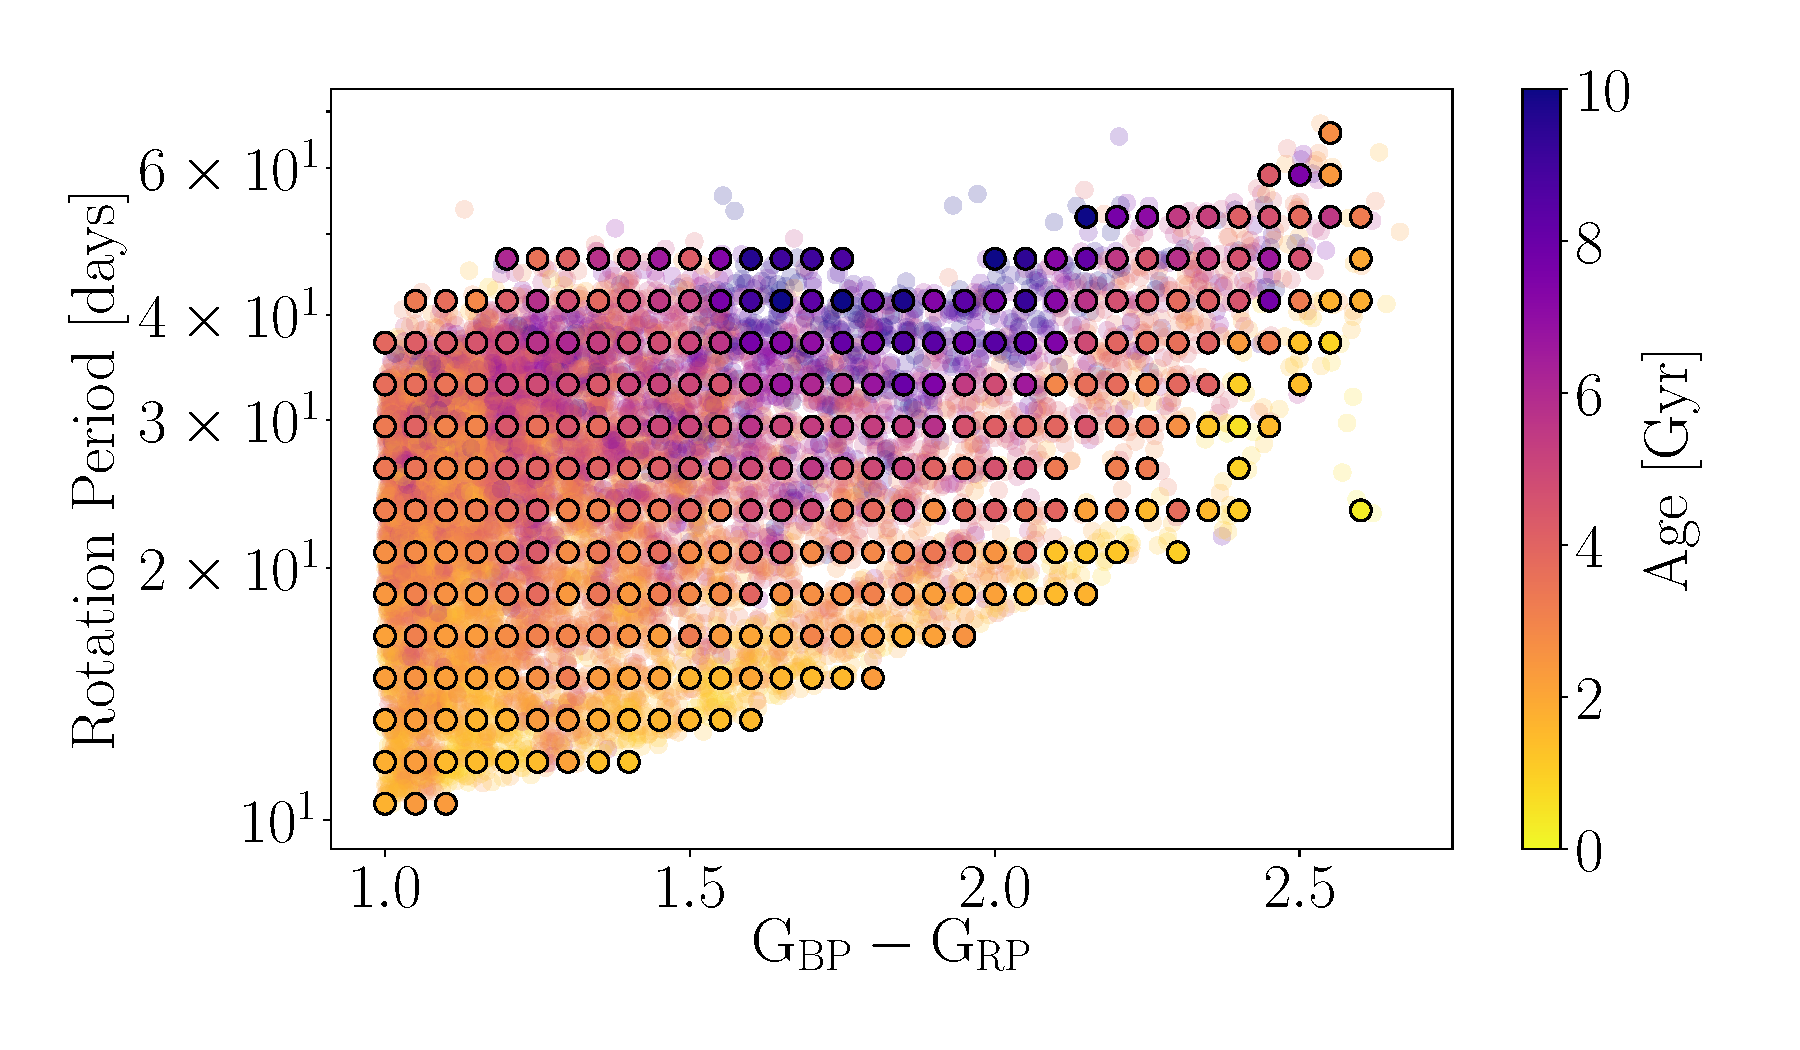
\includegraphics[width=1\textwidth]{grid_points}
    \label{fig:grid_points}
\end{figure}

\begin{figure}
\caption{
}
  \centering 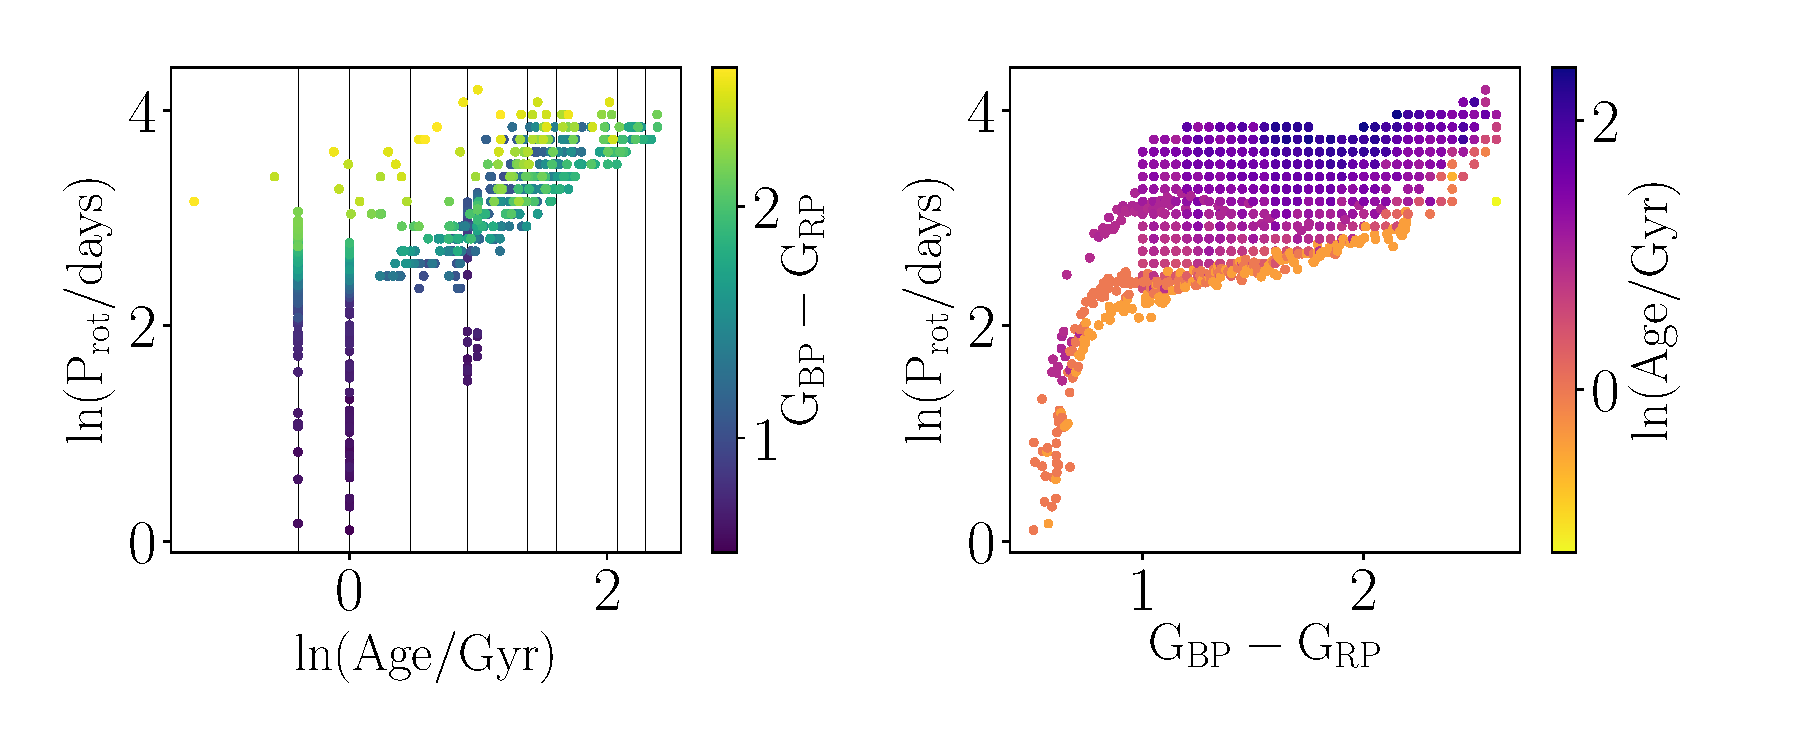
\includegraphics[width=1\textwidth]{gp_fit_data_multi-panel}
\end{figure}

\begin{figure}
\caption{
}
  \centering 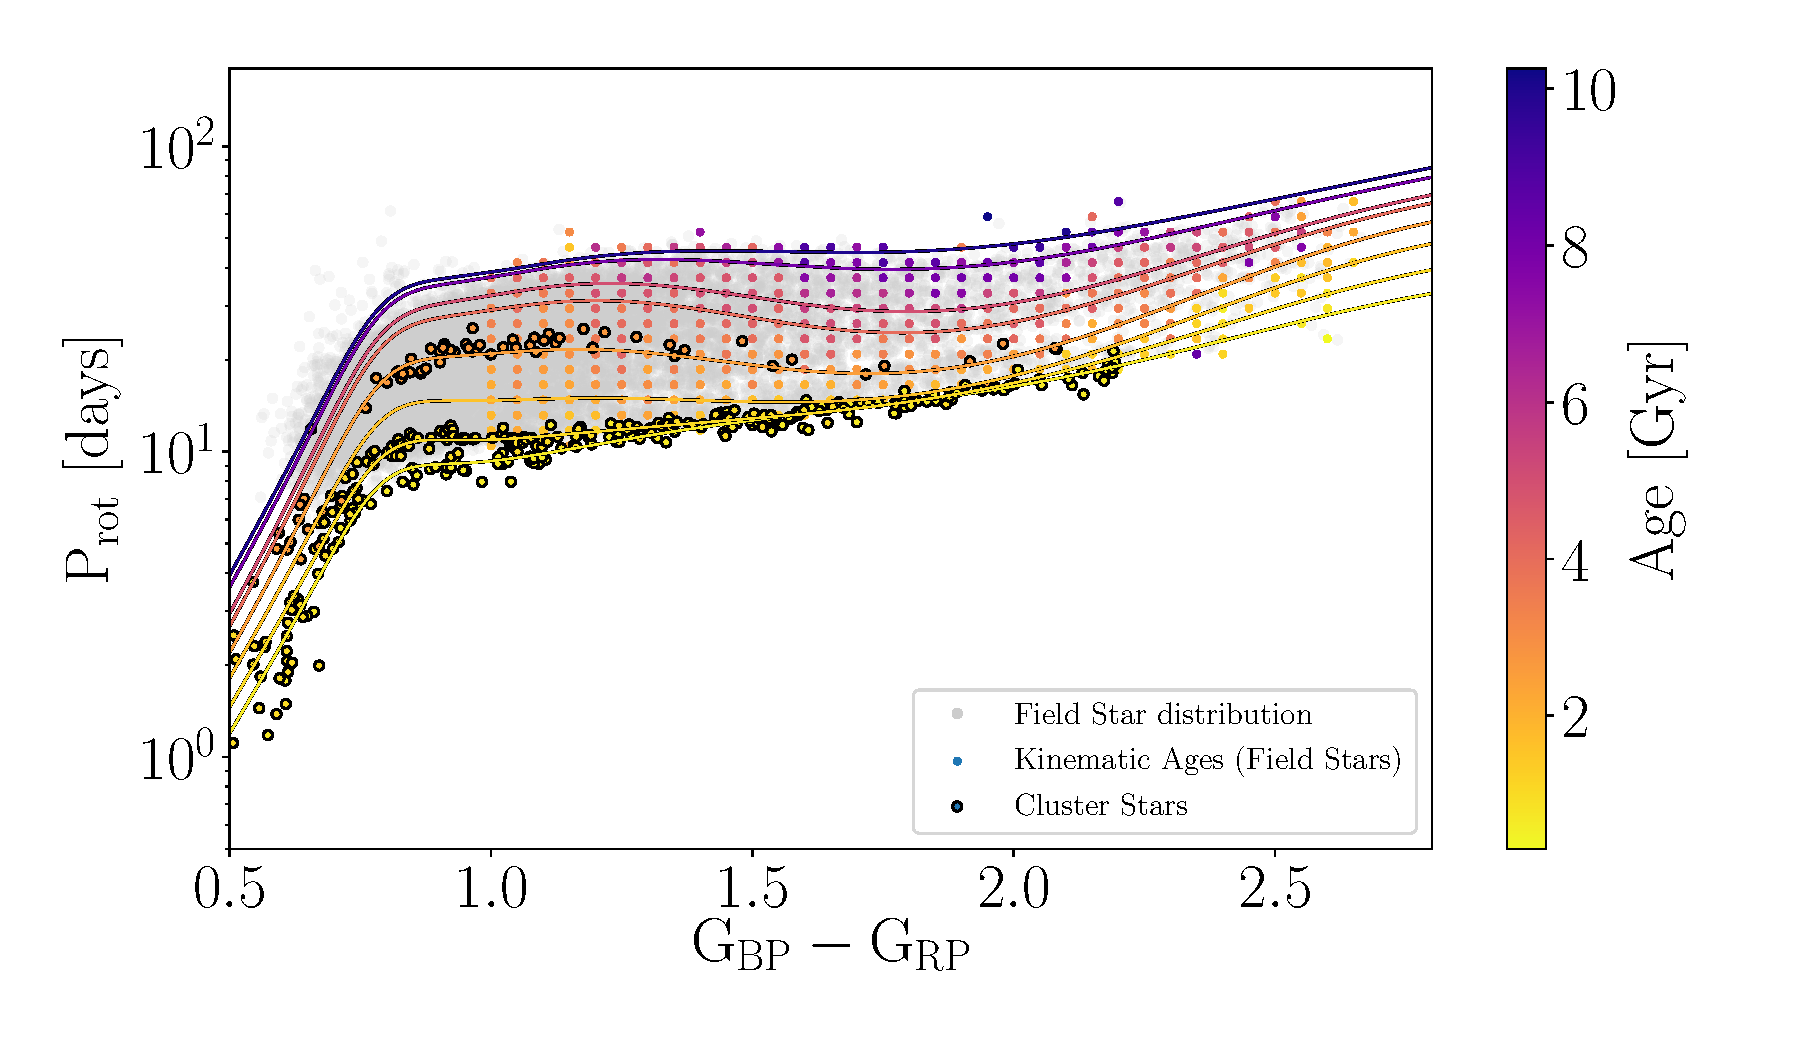
\includegraphics[width=1\textwidth]{gp_fit}
\end{figure}
